\chapter{The Graphical User Interface}
\label{cha:gui}

This chapter describes the RFSM IDE\footnote{Screenshots used in this chapter show the Windows
  version of the RFSM IDE. The IDE can also be built and used on Unix-based systems (Linux,
  MacOS).}. This IDE basically provides a Graphical user Interface (GUI) to the \verb|rfsmc|
compiler described in chapter~\ref{cha:rfsmc}.

\medskip
The GUI allows
\begin{itemize}
\item writing, reading and editing of RFSM programs,
\item generating and viewing graphical representations of these programs,
\item running simulations,
\item generating C, SystemC and VHDL code.
\end{itemize}

\medskip
\textbf{Note}. This chapter supposes that the IDE has been correctly installed. If not, refer to the
installation guide provided in the RFSM distribution.

\medskip
First, \textbf{launch the RFSM application} by clicking on its icon in the installation directory or
directly from the Windows \emph{Start} menu. 

\medskip
The application main window is shown in Fig.~\ref{fig:main-window}. 
The main elements are (with corresponding areas labeled in red in Fig.~\ref{fig:main-window}) :
\begin{enumerate}
\item a menubar,
\item a toolbar, containing four groups of buttons,
\item a sub-window for viewing project trees,
\item a sub-window for viewing input and output files,
\item a log area, displaying issued command and outputs from the compiler.
\end{enumerate}

\begin{figure}[h]
  \centering
  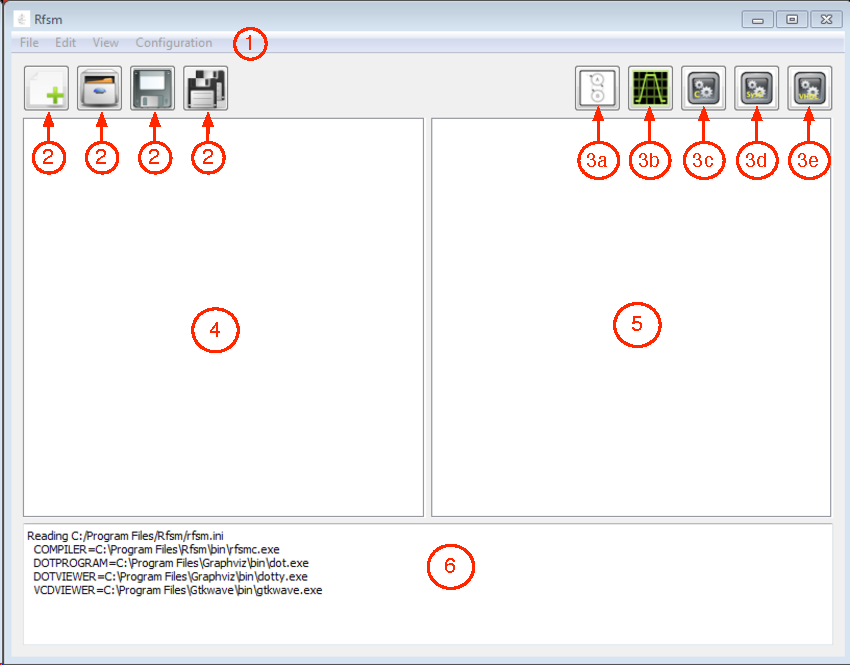
\includegraphics[width=0.75\textwidth]{figs/gui/mainwindow}
  \caption{Main window of the RFSM application}
  \label{fig:main-window}
\end{figure}

The buttons in the toolbar are respectively used to (from left to right, and grouped as depicted in
Fig.~\ref{fig:main-window})~:
\begin{enumerate}
\item 
  \begin{itemize}
  \item open an existing project
  \item open an existing file
  \item create a new file
  \end{itemize}
\item 
  \begin{itemize}
  \item generate a graphical representations of the currently selected source file
  \item generate C code from the currently selected source file
  \item generate SystemC code from the currently selected source file
  \item generating VHDL code from the  currently selected source file
  \end{itemize}
\item 
  \begin{itemize}
  \item generate a graphical representations of the current project
  \item generate C code from the current project
  \item generate SystemC code from the current project
  \item generating VHDL code from the current project
  \item simulate the current project
  \end{itemize}
\end{enumerate}

\section{Configuration}
\label{sec:gui-configuration}

Invoke the [\textsf{Configuration:Compiler and Tools}] menu item and check that the specified paths
are right (see Fig.~\ref{fig:config-window}). They should respectively point to 
\begin{itemize}
\item the location of the \texttt{rfsmc} compiler (\verb|<install>/bin/rfsmc|, where
  \verb|<install>| is the RFSM installation directory, as specified during the installation
  process),
\item the location of the program to invoke for processing \verb|.dot| files, 
\item the location of the program to invoke for viewing \verb|.dot| files, 
\item the location of the program to invoke for viewing \verb|.vcd| traces. 
\end{itemize}
If the specified paths are not correct\footnote{This may be the case, for example, if you have
  changed the program to view graphs and/or images since RFSM was installed.}, adjust them and click \textsc{Ok}.

\begin{figure}[h]
  \centering
  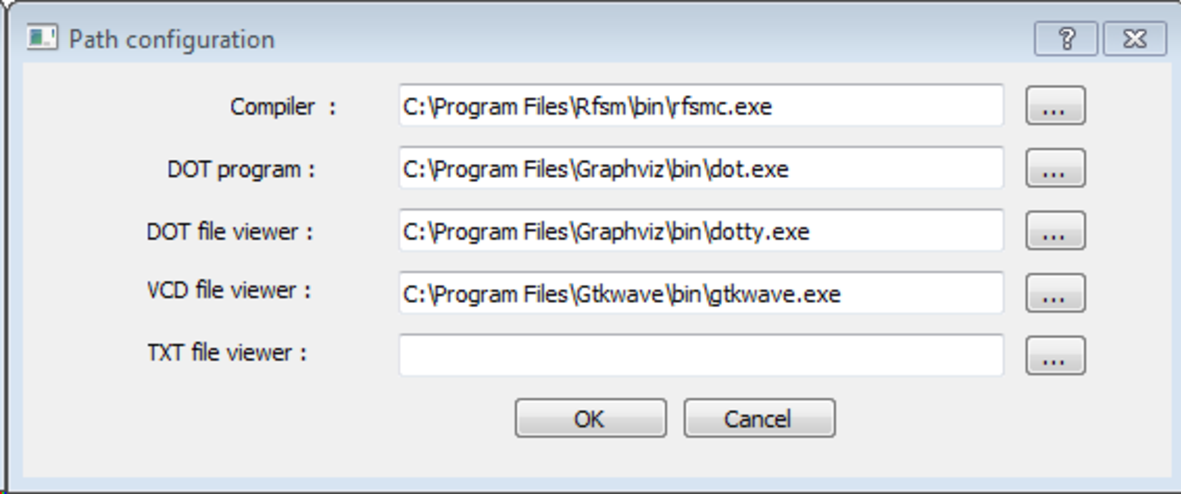
\includegraphics[width=0.75\textwidth]{figs/gui/pathconfig}
  \caption{Path configuration window}
  \label{fig:config-window}
\end{figure}

\section{Single file mode}
\label{sec:gui-single-file-mode}

The GUI supports two modes of operation~: \emph{single file mode} and \emph{project mode}. 

In \emph{single file mode}, the compiler is invoked on a single source file, whis is supposed to
contain the description of a FSM model, to produce a DOT representation of the model or the C,
SystemC or VHDL corresponding code.

Source files (\verb|.fsm|) can be created by clicking on the \textsf{New File} button\footnote{First
  group, third button in the toolbar.} or by invoking the corresponding item of the \textsf{File}
menu. Existing source file can opened by clicking on the \textsf{Open file} button\footnote{First
  group, second button} or, similarly, by invoking the corresponding item of the \textsf{File} menu.

Once opened, source files appear in a new tab in the right subwindow (numbered 4 in
Fig.~\ref{fig:main-window}) and can can be freely edited and saved. 

Fig.~\ref{fig:open-file} shows the GUI after
opening the source file \verb|ctlr.fsm|, located in directory \texttt{examples/single/mousectlr} of
the distribution.

\begin{figure}[h]
  \centering
  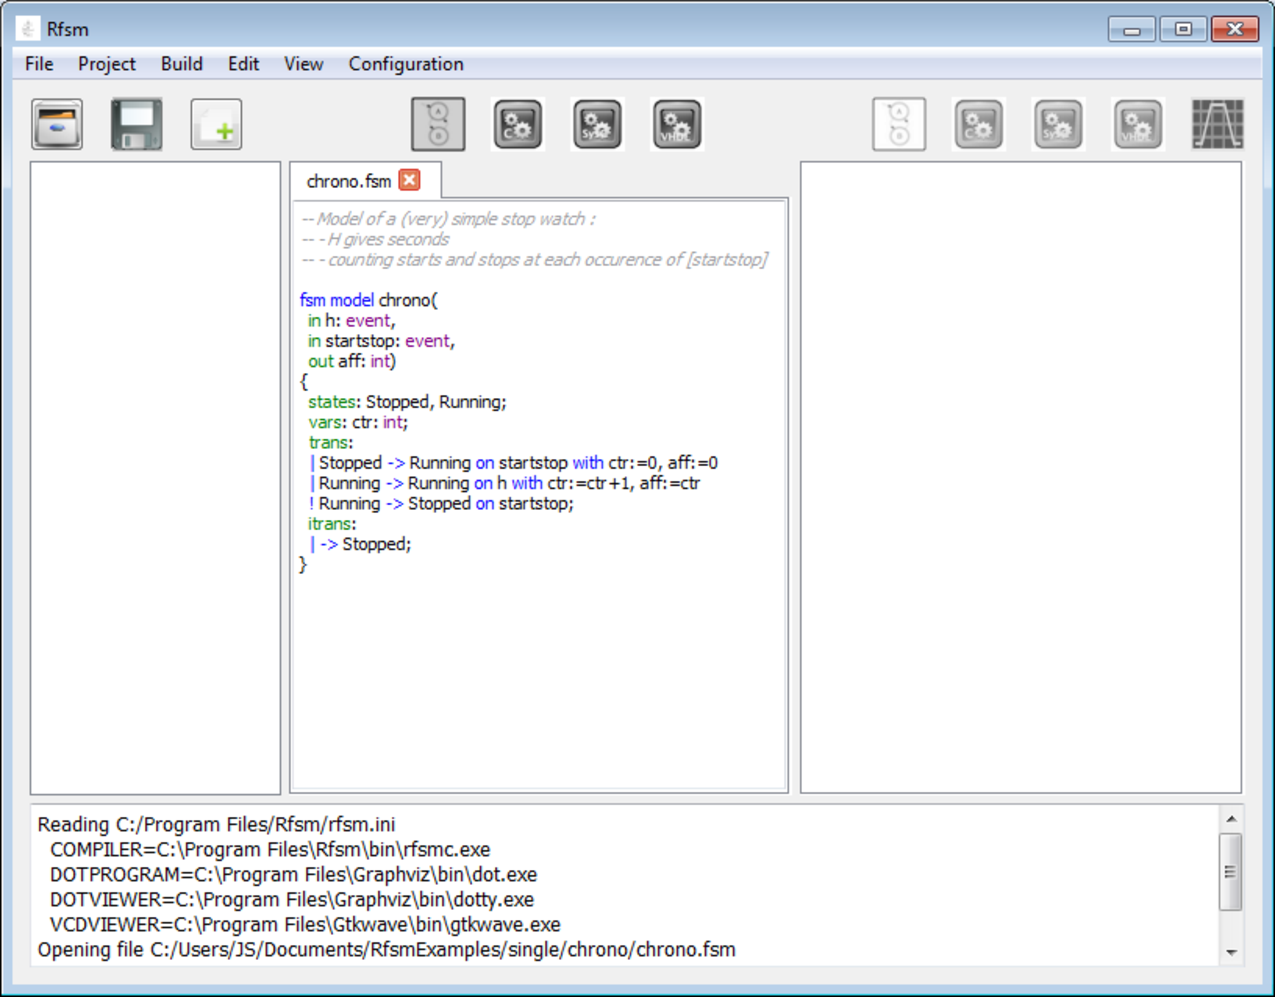
\includegraphics[width=0.75\textwidth]{figs/gui/open-file}
  \caption{Opening a source file}
  \label{fig:open-file}
\end{figure}

\medskip
To \textbf{generate the graphical representation of the program}, click on the \textsf{Graph} button
(second group, first button in toolbar) or invoke the \textsf{Build DOT representation for file}
item in the \textsf{Build} menu. This will
\begin{itemize}
\item invoke the \verb|rfsmc| compiler with the adequate option(s),
\item generate the \texttt{.dot} result file (in the same directory as the source file),
\item view this result by invoking the graph visualisation program specified in 
  [\textsf{Configuration : Compiler and Tools}] window.
\end{itemize}

The result for the previously opened source file is displayed in Fig.~\ref{fig:make-dot}.

\begin{figure}[h]
  \centering
  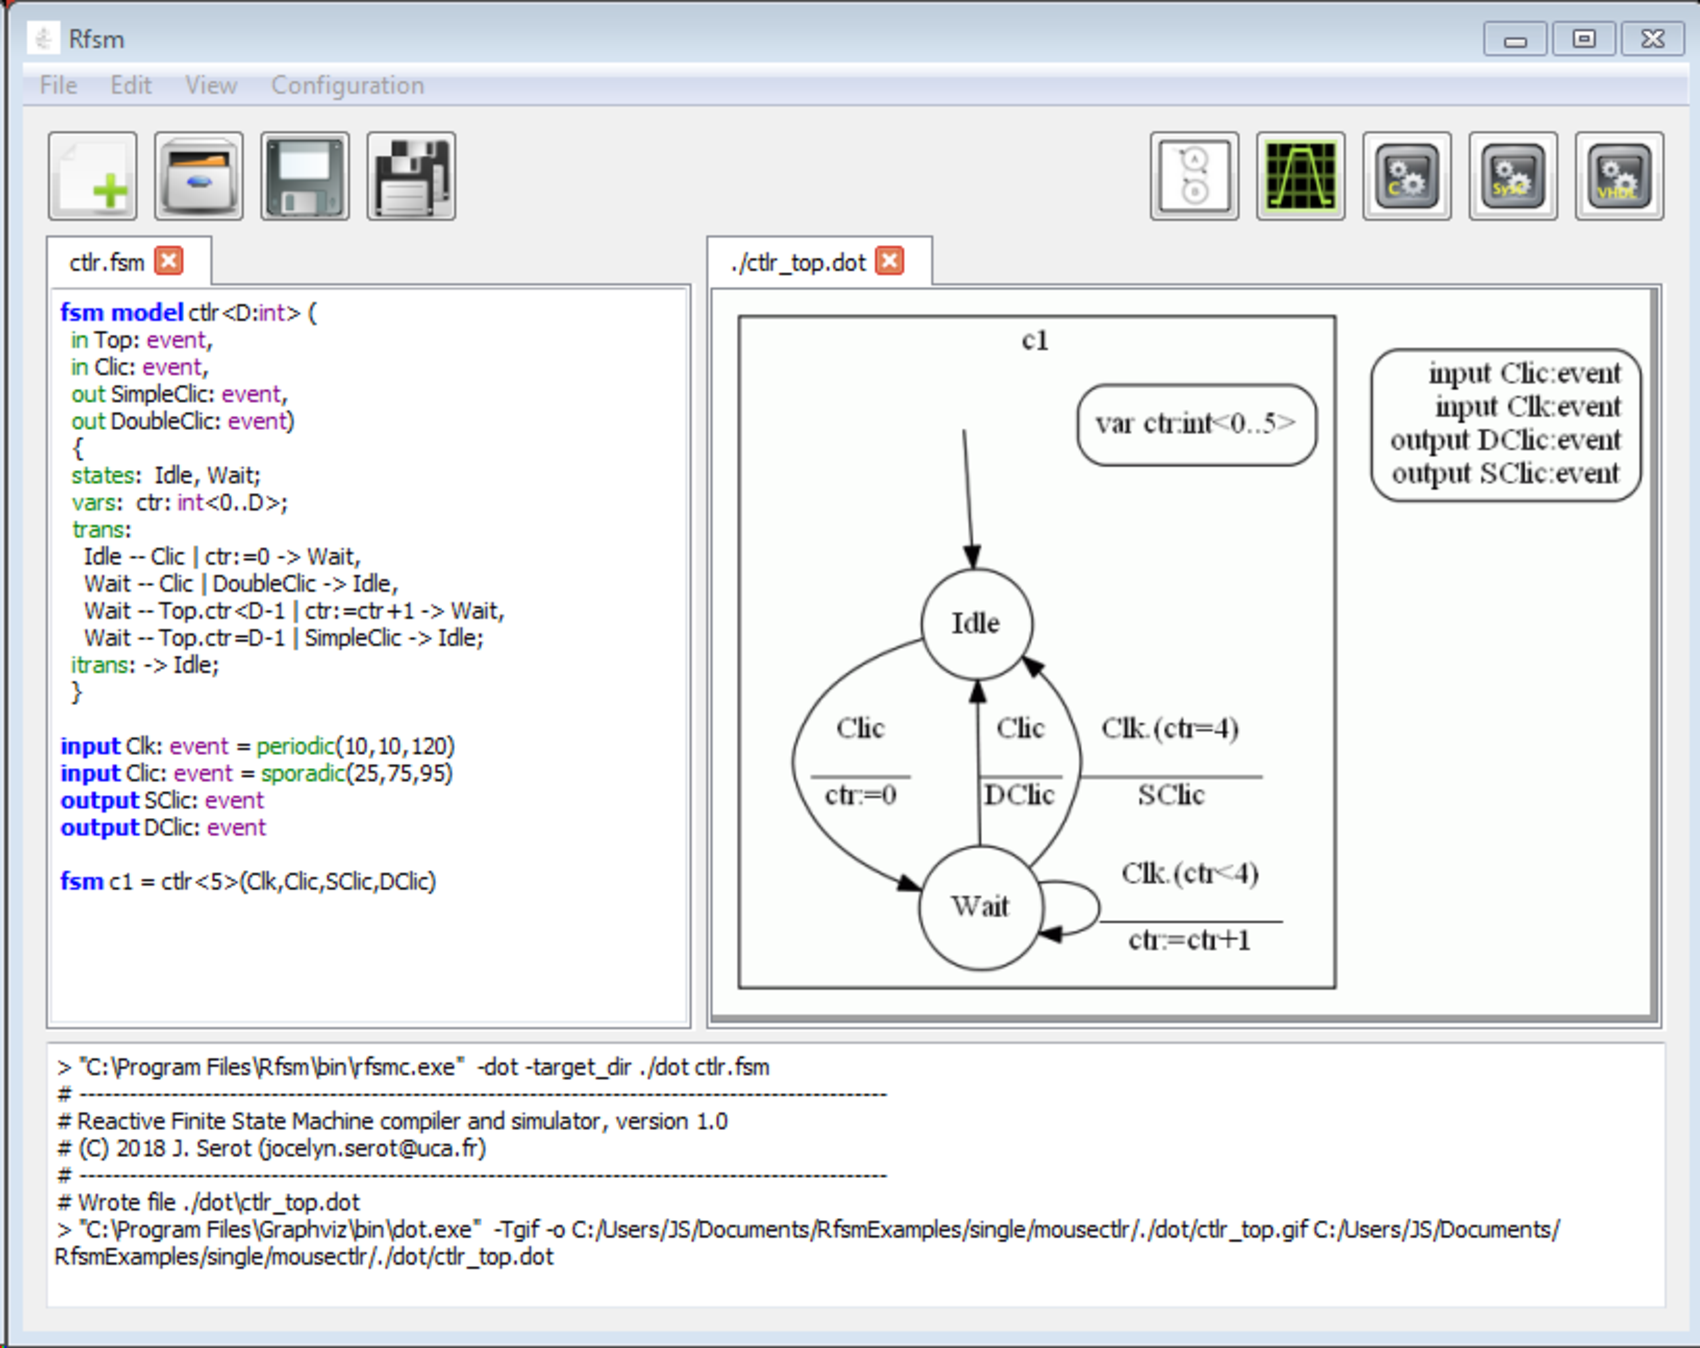
\includegraphics[width=0.75\textwidth]{figs/gui/make-dot}
  \caption{Viewing the graphical representation of the program}
  \label{fig:make-dot}
\end{figure}

\medskip For \textbf{generating the C, SystemC or VHDL} code, click on the corresponding buttons
(second, third and fourth button in the second group of the toolbar) or invoke the corresponding
items in the \textsf{Build} menu. The result files will be generated in sub-directories named
\verb|./ctask|, \verb|./systemc| and \verb|./vhdl| and displayed as separate tabs, as
illustrated in Fig.~\ref{fig:make-systemc}, for example.

\begin{figure}[h]
  \centering
  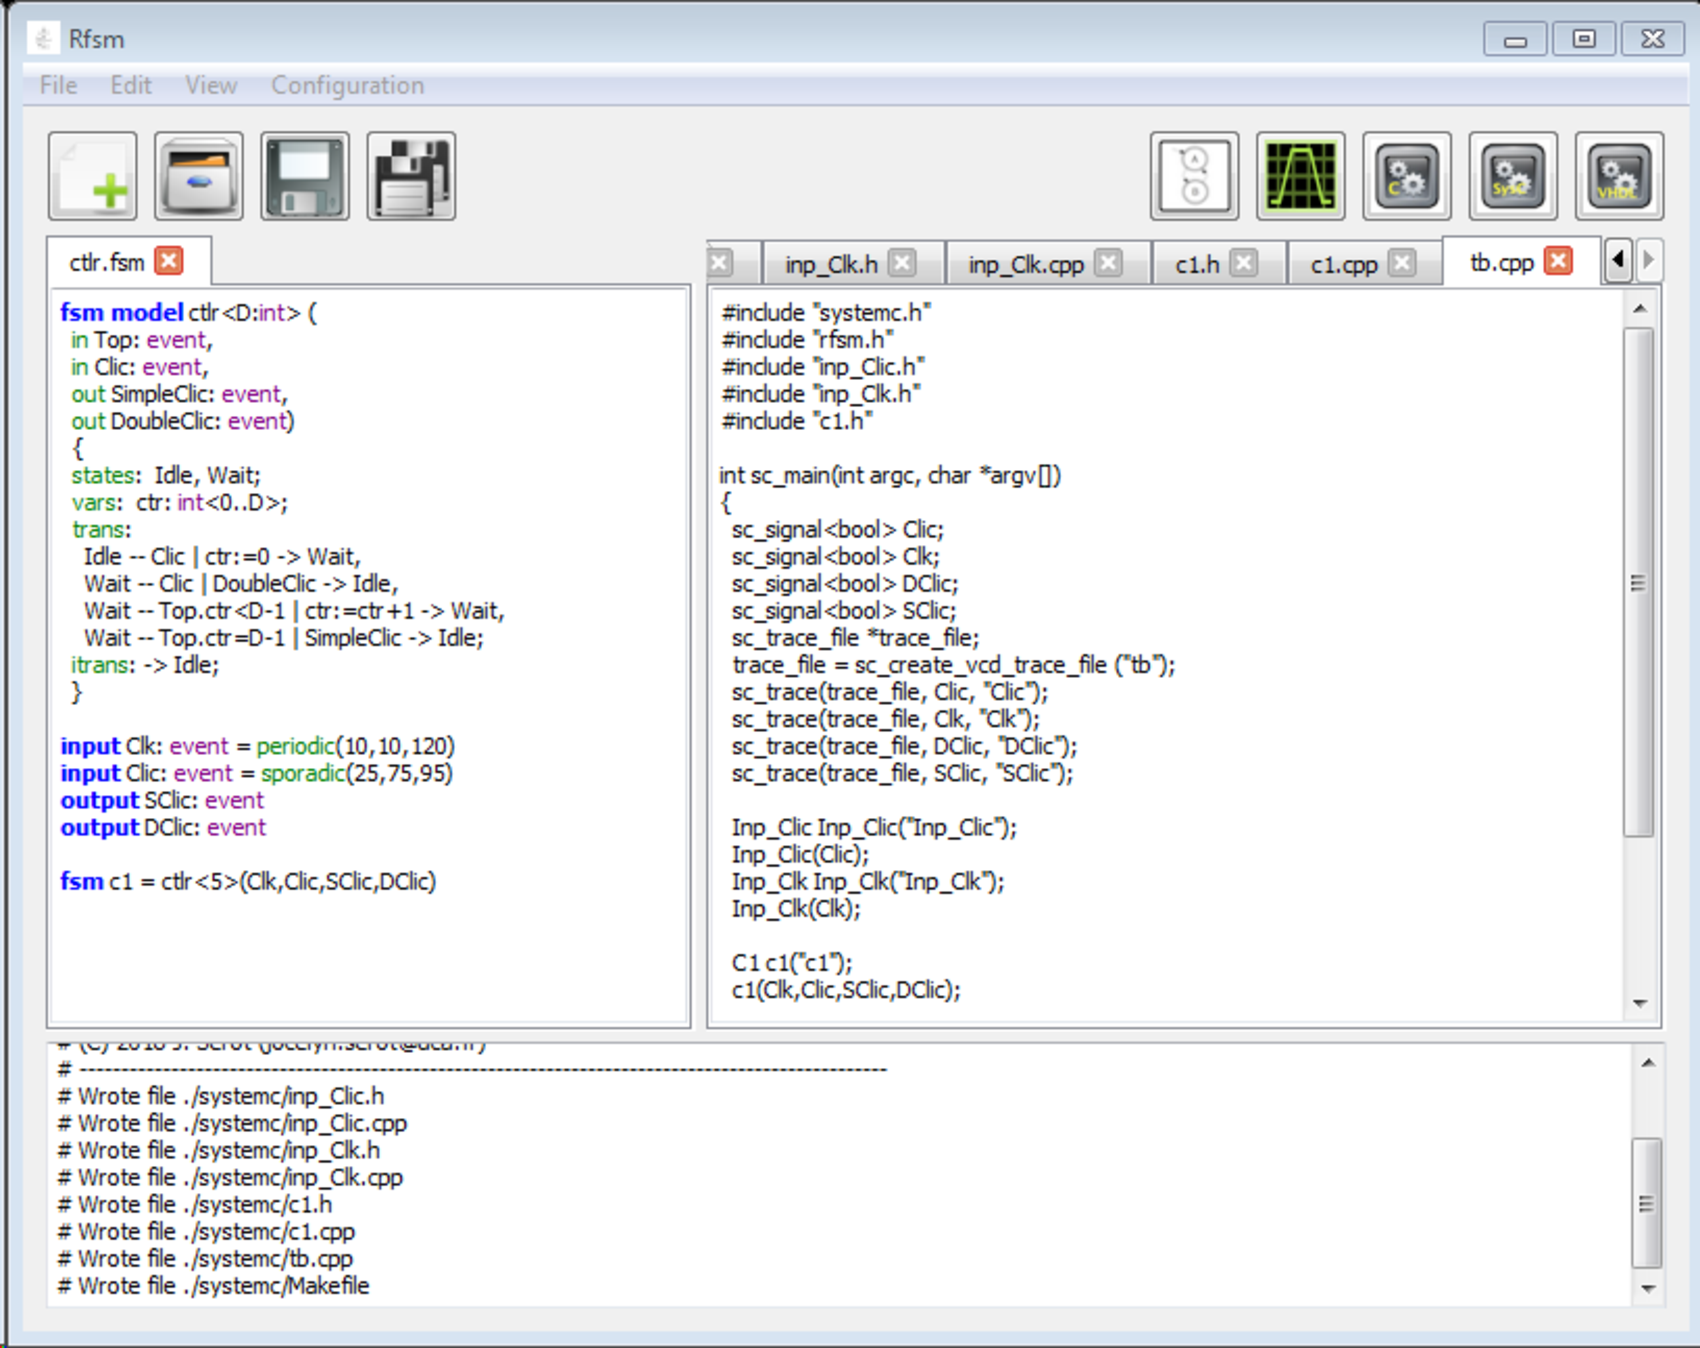
\includegraphics[width=0.75\textwidth]{figs/gui/make-systemc}
  \caption{After generating SystemC code}
  \label{fig:make-systemc}
\end{figure}

\section{Project mode}
\label{sec:gui-project-mode}

In \emph{project mode}, the GUI can work on multiple source files and remember specific compiler
options using the project description files (\verb|.pro|) introduced in Sec~\ref{sec:rfsmmake}.

This is illustrated in Fig.~\ref{fig:open-project}, which depicts the GUI after opening the project
described by the file \verb|main.pro| located in the directory \texttt{examples/single/mousectlr}.
This project is composed of two source files~: the file \verb|ctlr.fsm|, which contains a FSM
model\footnote{This file is the same as the one used as an example in
  Sec.~\ref{sec:gui-single-file-mode}.} and the file \verb|main.fsm|, which contains a
\emph{testbench} for this model. These files are shown on the tree view in the left sub-window,
along with the sub-directories in which the compilation results will be written. 

\begin{figure}[h]
  \centering
  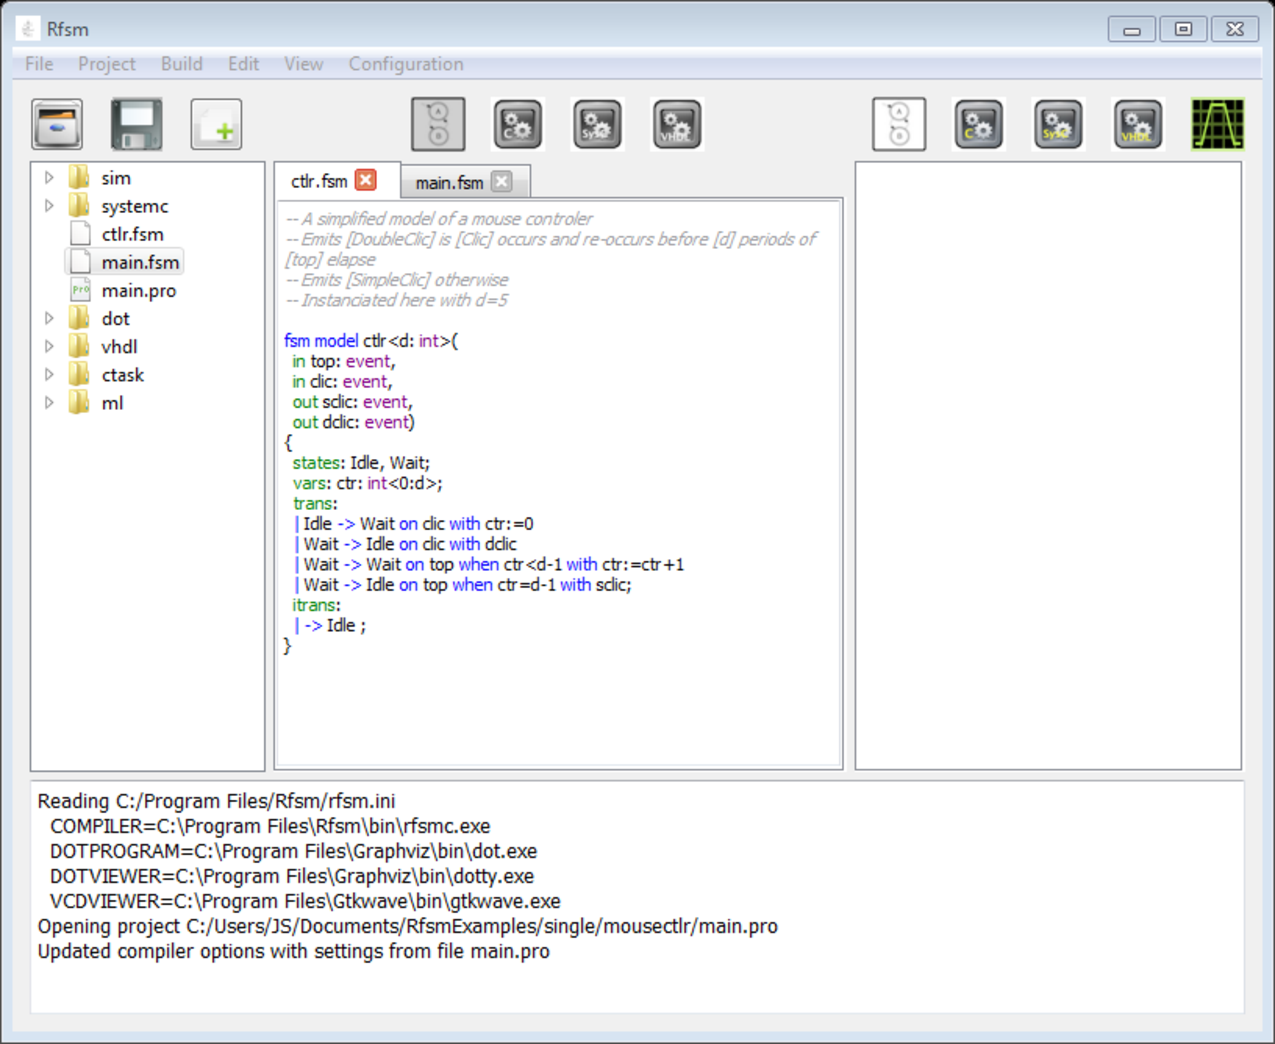
\includegraphics[width=0.75\textwidth]{figs/gui/open-project}
  \caption{Opening a project}
  \label{fig:open-project}
\end{figure}

Invoking the \textsf{Build ... for project} items of the \textsf{Build} menu\footnote{Or the
  corresponding buttons in the toolbar (first, second, third and fourth of the second group
  respectively.} will build the corresponding representations (DOT, C, SystemC or VHDL) of the
program described by the project.  For example, Fig.~\ref{fig:make-dot-project} gives the state of
the GUI after building the DOT representation of the above-mentioned project. Note that two
\verb|.dot| files have here been generated~: one the for the FSM model described in file
\verb|ctlr.fsm| and another for the \emph{testbench} described in file \verb|main.fsm|. Each
representation is displayed in a separate tab of the sub-window on the
right. Fig.~\ref{fig:make-dot-project} shows the tab associated to the file \verb|main.dot|. 

\begin{figure}[h]
  \centering
  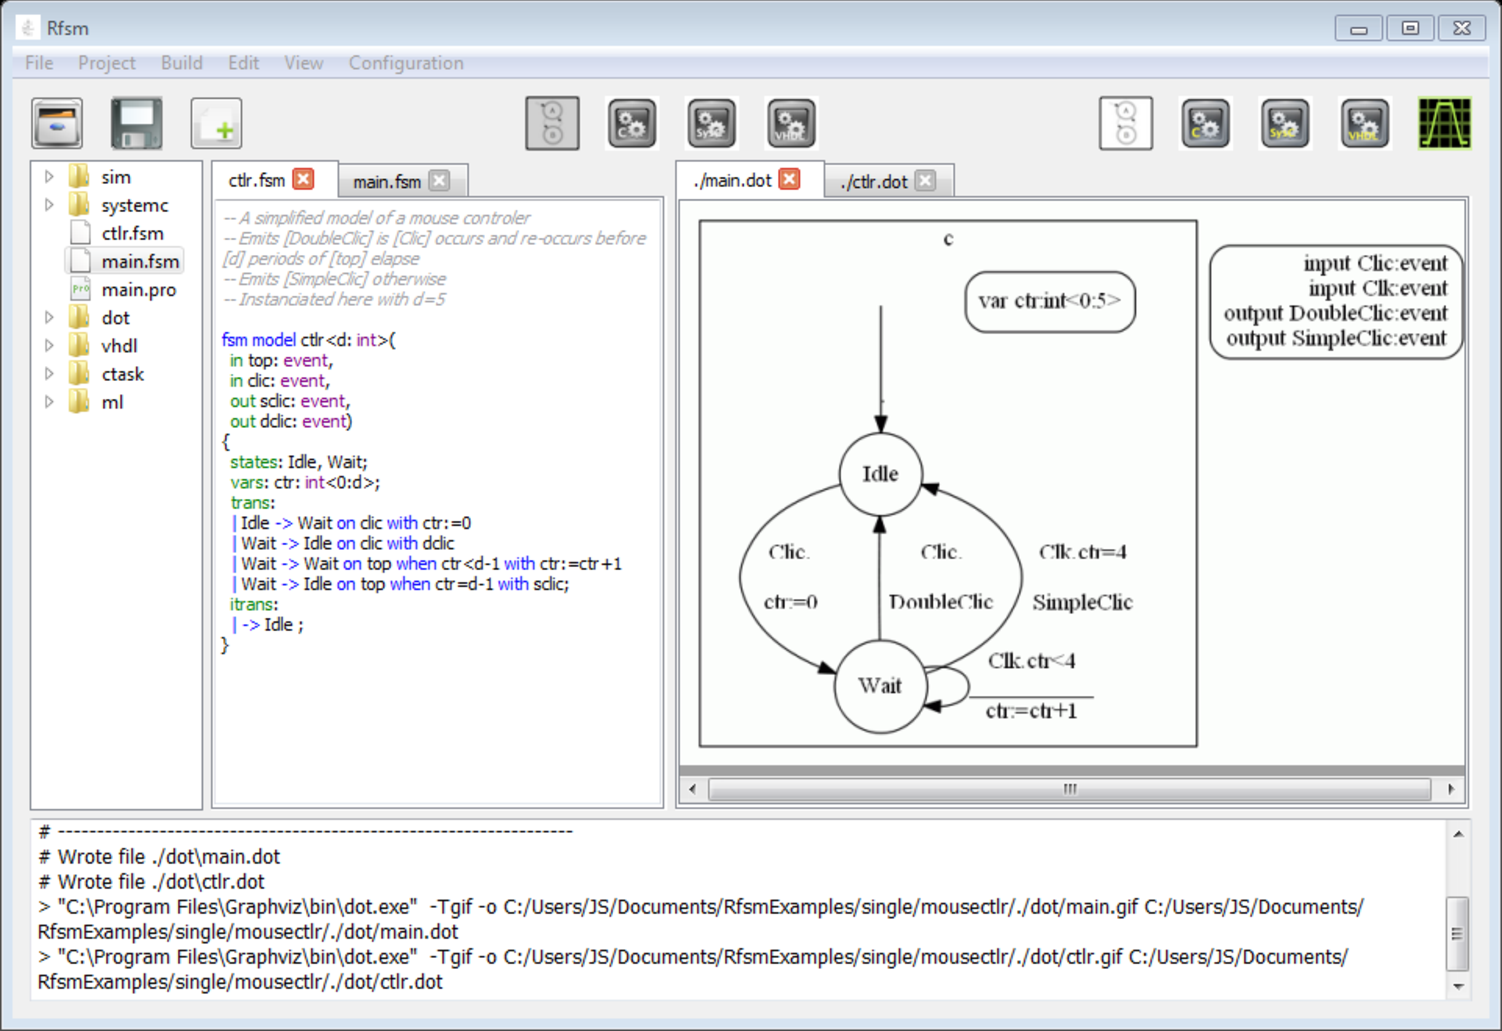
\includegraphics[width=0.75\textwidth]{figs/gui/make-dot-project}
  \caption{After building the DOT representation of the project introduced in
    Fig.~\ref{fig:open-project}}.
  \label{fig:make-dot-project}
\end{figure}


\medskip
In project mode, the program described by the project can also be \textbf{simulated} by clicking on
the corresponding button in the toolbar\footnote{Last button on the right, with the green
  waveform.}. This runs the program, generates results in a VCD file and launch the VCD viewer specified in 
  [\textsf{Configuration : Compiler and Tools}] window. In the case of the program introduced in
  Fig.~\ref{fig:open-project}, this is illustrated in Fig.~\ref{fig:make-sim} (with the
  \verb|gtkwave| VCD viewer).

\begin{figure}[h]
  \centering
  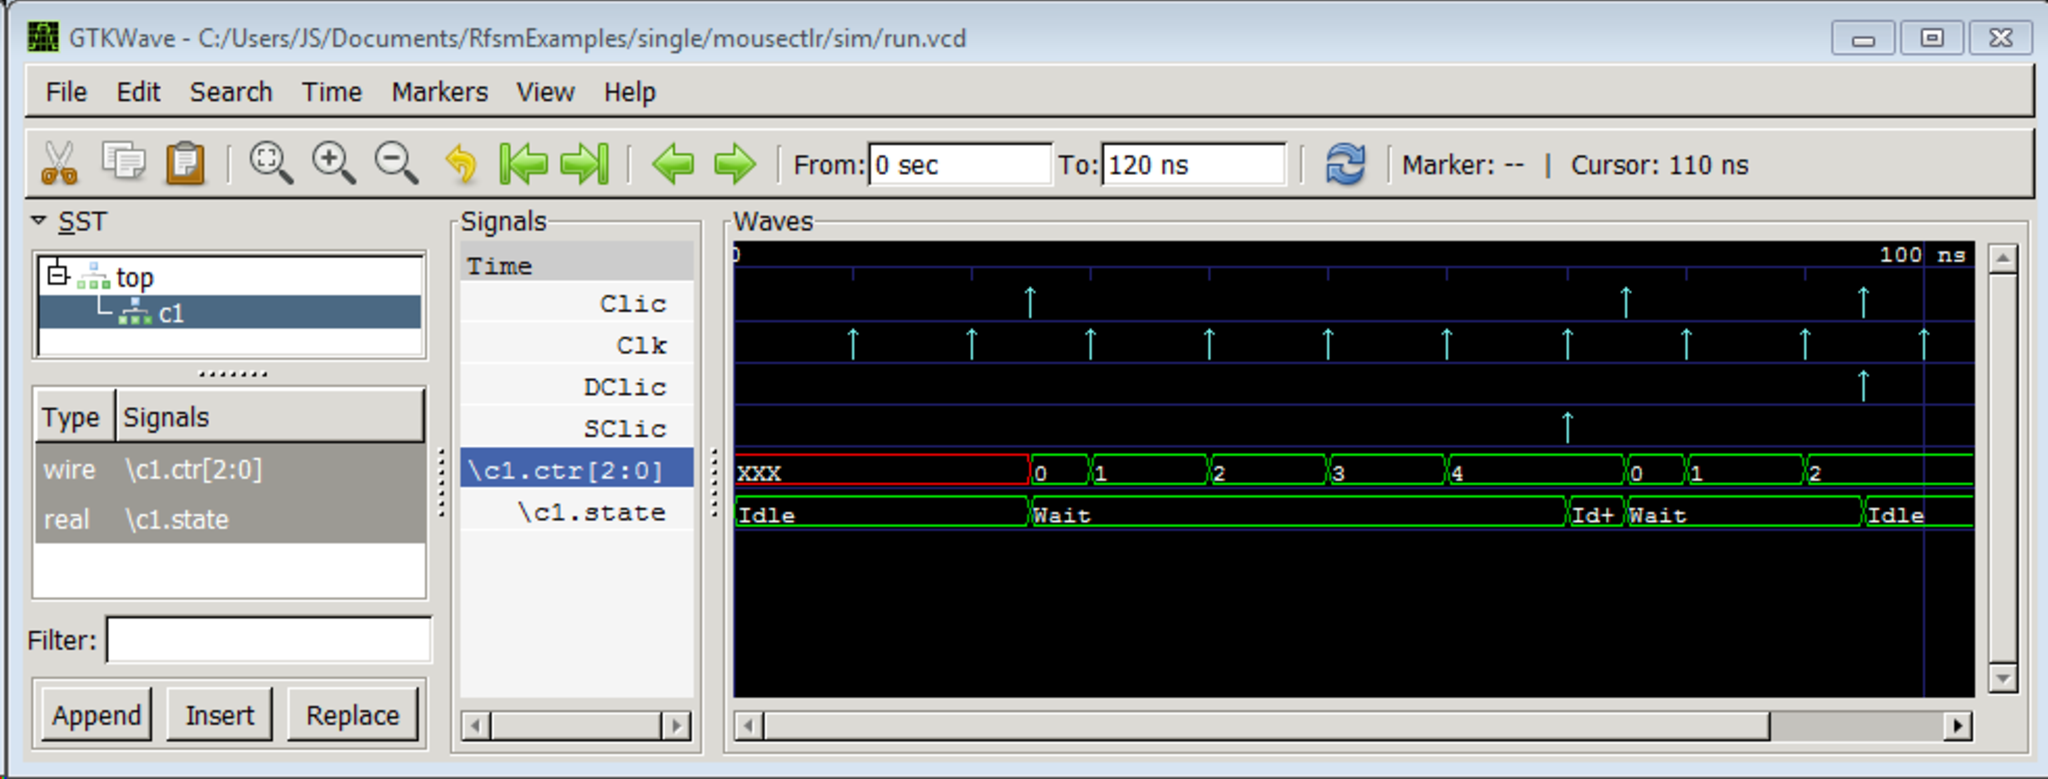
\includegraphics[width=0.75\textwidth]{figs/gui/make-sim}
  \caption{Viewing the simulation result}
  \label{fig:make-sim}
\end{figure}


\section{Setting options}
\label{sec:gui-setting-options}

TBW

% Options to be passed to RFSM compiler can be set and inspected by invoking \textsf{Compilater options} item of the
% \textsf{Configuration} menu, as illustrated in Fig.~\ref{fig:options}. These options are
% documented in Appendix B.

% \begin{figure}[h]
%   \centering
%   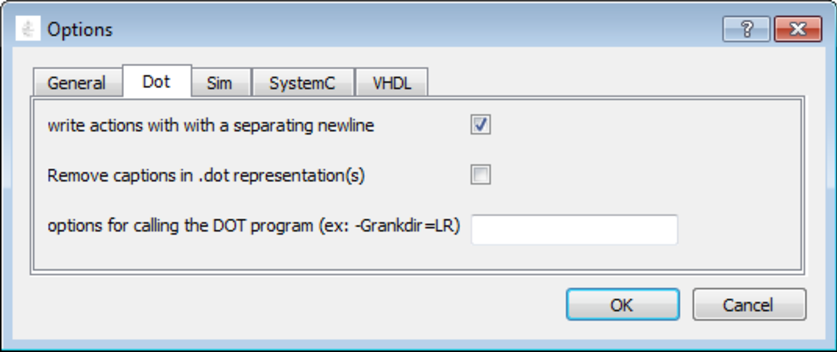
\includegraphics[width=0.75\textwidth]{figs/gui/options}
%   \caption{The options setting dialog}
%   \label{fig:options}
% \end{figure}

%%% Local Variables:
%%% mode: latex
%%% TeX-master: "rfsm"
%%% End:
